\section{Get into the quntum world}\SectionRule
    \subsection{\hfill \small Monday Sep 2}
    \subsection{\hfill\small Tuesday Sep 3}
    \subsubsection*{Bohr-Sommerfeld Quantization (Old quantum theory)}
    \[
        \oint p \,dq = nh
    \]
    While $p$ is the momentum of a particle, which is a function of position of particle $q$. This equation constrains the movement of a particle in a specific potential field V(q).
    \subsection{\hfill \small Friday Sep 6}
    \subsubsection*{Born Statistical Interpretation of Wave Function}
    The wave function $\Psi (x,t)$ discribes the "Amplitude" of the probability finding the paticle at coordinate(x,t). While the probability density equals amplitude squared.

    That is, the probability finding the particle among $x\in [a,b]$ at time $t_0$ is discribed as:
    \begin{equation*}
        P(x\in [a,b],t=t_0)=\int^{b}_{a}|\psi|^{2}dx=\int^{b}_{a}\psi^*\psi dx
    \end{equation*}

    Or, to say, the \textit{Probability Density} can be written as:
    \begin{equation*}
        p(x,t)=|\psi(x,t)|^2=\psi^{*}(x,t)\psi(x,t)
    \end{equation*}
    
    \subsection*{Homework}
        \subsubsection*{[week1 hw1]}
        \subsubsection{[Thinking][Optional] A Brief History of Clues}
        {\color{hwSolution}
            \textbf{PENDING: This part will be done later this week.}
        }
        \subsubsection{Caculate wave length of an electron after a 1000V potential field}
        
        {\color{hwSolution}
        Utilizing \textit{\textbf{de Broglie wave}} equation (ignoring relativity effect):
        \begin{align*}
            Energy~obtained~by~this~electron:&& E = q\cdot U &= 1000\,eV\\
            Corresponding~momentum~of~this~electron:&& p &= \sqrt{2m\cdot E}\\
            Wave~length~of~this~electorn:&& \lambda &= \dfrac{h}{p}\\
            &&&=\dfrac{6.626\times10^{-34}}{\sqrt{2\times 9.1\times 10^{-31}\times 1000\times 1.6\times10^{-19}}}\\
            &&&=3.88\times 10^{-9}\,m
        \end{align*}
        }

        \subsubsection{Derivation of Klein-Gordon equation}

        {\color{hwSolution}
            \textbf{PENDING: This part will be done later this week.}
        }
        \subsubsection*{[week1 hw2]}
        \subsubsection{Griffiths 1.2}
        \noindent{
            (a) Find the standard deviation of the distribution in Example 1.1.
        }
        
        {\color{hwSolution}
            First caculate the probability of finding this object at position $x$, represented by $\rho(x)$:
            \begin{align*}
                total~travel~time~T=\sqrt{\dfrac{2\,h}{g}}\\
                dt = \dfrac{dx}{v} = \dfrac{1}{\sqrt{2gx}}\,dx\\
                \rho(x) = \dfrac{dt}{T\,dx} = \dfrac{1}{2\sqrt{hx}}
            \end{align*}

            Accoring to statistics:

            \begin{tabularx}{\linewidth}{X|X}
                {\begin{align*}
                \<x\>^2   &= \left(\int_0^h x\cdot\rho(x)\,dx\right)^2\\
                &= \left(\int_0^h \dfrac{x}{2\sqrt{hx}}\,dx\right)^2\\
                &= \dfrac{h^2}{9}\\
                \end{align*}}
                &
                {\begin{align*}
                \<x^2\>   &= \int_0^h x^2\cdot\rho(x)\,dx\\
                &= \int_0^h \dfrac{x^2}{2\sqrt{hx}}\,dx\\
                &= \dfrac{h^2}{5}
                \end{align*}}
            \end{tabularx}

            Hence:
            \begin{align*}
                \delta  &= \sqrt{\<x^2\> - \<x\>^2}\\
                        &= \dfrac{2}{3\sqrt{5}}\,h
            \end{align*}
        }

        \noindent{
            (b) What is the probability that a photograph, selected at ramdom, would show a distance $x$ more than one standard deviation away from the average?
        }

        {\color{hwSolution}
            We have known that the average is $\<x\>=\frac{h}{3}$, and the standard deviation is $\delta=\frac{2}{3\sqrt{5}}\,h$. We now want to know the probability of finding x among $0<x<\<x\>-\delta$ or $\<x\>+\delta < x < h$:
            \begin{align*}
                P   &= \int_0^{\<x\>-\delta} \rho(x)\,dx + \int_{\<x\>+\delta}^h \rho(x)\,dx\\
                    &= 1 - \int_{\<x\>-\delta}^{\<x\>+\delta} \rho(x)\,dx\\
                    &= 1 - \dfrac{1}{\sqrt{h}}\left(
                        \left. \sqrt{x}\right|_{\frac{5-2\sqrt{5}}{15}\,h}^{\frac{5+2\sqrt{5}}{15}\,h}
                    \right)\\
                    &= 1 - \left(\sqrt{\dfrac{5+2\sqrt{5}}{15}}-\sqrt{\dfrac{5-2\sqrt{5}}{15}}\right)\\
                    &\approx 0.39
            \end{align*}
        }

        \subsubsection{Griffiths 1.4}
        \noindent{
            At time $t=0$ a particle is represented by the wave function
            \begin{equation*}
                \Psi(x,0)=
                \left\{\begin{array}{ll}
                    A\dfrac{x}{a}, & if~~0\leq x\leq a, \\
                    \\
                    A\dfrac{(b-x)}{(b-a)}, & if~~a\leq x\leq b, \\
                    \\
                    0, & otherwise,
                \end{array}
                \right.
            \end{equation*}
            where $A,a$ and $b$ are constants.
        }
        
        \noindent{
            (a) Normalize $\Psi$ (that is, find A in terms of $a$ and $b$)
        }

        {\color{hwSolution}
            The integral of $|\Psi|^2$ in all space is:
            \begin{align*}
                \int_{-\infty}^{+\infty}\Psi^*\Psi\,dx
                &= \int_0^a A^2\,\dfrac{x^2}{a^2}\,dx
                +  \int_a^b A^2\,\dfrac{\left(b-x\right)^2}{\left(b-a\right)^2}\,dx\\
                &= A^2\left(\dfrac{a}{3}+\dfrac{b-a}{3}\right)\\ 
                &= \dfrac{1}{3}\,A^2b\\
                &= 1
            \end{align*}
            Hence:
            \[A = \sqrt{\dfrac{3}{b}}\]
        }

        \noindent{
            (b) Sketch $\Psi (x,0)$, as a function of $x$.
        }

        {\color{hwSolution}
            Let $a=1,~b=3~\Rightarrow A=1$:
        }
        
        \begin{center}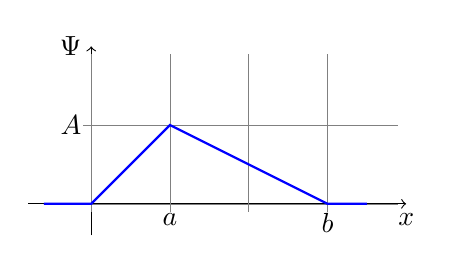
\begin{tikzpicture}
            \draw[thin,->](-0.8,0)--(4,0) node[below]{$x$};
            \draw[thin,->](0,-0.4)--(0,2) node[left]{$\Psi$};
            \draw[very thin,color=gray] (-0.1,-0.1) grid (3.9,1.9);
            \draw[blue,thick](-0.6,0)--(0,0)--(1,1)--(3,0)--(3.5,0);
            \path   (0,1) node[left]{$A$}
                    (1,0) node[below]{$a$}
                    (3,0) node[below]{$b$};
        \end{tikzpicture}\end{center}

        \noindent{
            (c) Where is the particle most likely to be found, at $t=0$?.
        }

        {\color{hwSolution}
            Obviously, at $x=a$.
        }

        \noindent{
            (d) What is the probability of finding the particle to the left of $a$? Check your result in the limiting cases $b=a$ and $b=2a$.
        }

        {\color{hwSolution}
        \begin{center}\begin{tabularx}{\linewidth}{X|X}
            In case of~~$b=a$: & In case of~~$b=2a$:\\
            {\begin{align*}
                A &= \sqrt{\dfrac{3}{b}}
                = \sqrt{\dfrac{3}{a}}\\
                P &= \int_0^a \dfrac{3}{a} \,\left(\dfrac{x}{a}\right)^2\,dx
                = 1
            \end{align*}}
            &
            {\begin{align*}
                A &= \sqrt{\dfrac{3}{b}}
                = \sqrt{\dfrac{3}{2a}}\\
                P &= \int_0^a \dfrac{3}{2a} \,\left(\dfrac{x}{a}\right)^2\,dx
                = \dfrac{1}{2}
            \end{align*}}
        \end{tabularx}\end{center}
        }

        \noindent{
            (e) What is the expectation value of $x$?
        }

        {\color{hwSolution}
            \begin{align*}
                \<x\> &= \dfrac{3}{b}\left(
                    \int_0^a x\cdot\dfrac{x^2}{a^2}\,dx
                    +
                    \int_a^b x\cdot\dfrac{(b-x)^2}{(b-a)^2}\,dx
                    \right)
                    = \dfrac{3}{b}\left(\dfrac{a^2}{4}+\dfrac{b^4-3a^4+8a^3b-6a^2b^2}{12\,(b-a)^2}\right)\\
                    &= \dfrac{3a^2(b-a)^2+b^4-3a^4+8a^3b-6a^2b^2}{4b\,(b-a)^2}
                    = \dfrac{\bcancel{3a^4}+3a^2b^2-6a^3b+b^4-\bcancel{3a^4}+8a^3b-6a^2b^2}{4b\,(b-a)^2}\\
                    &= \dfrac{\bcancel{b}(b^3+2a^3-3a^2b)}{4\,\bcancel{b}\,(b-a)^2}
                    = \dfrac{(b-a)^{\bcancel{3}}+3a\bcancel{(b-a)^2}}{4\bcancel{(b-a)^2}}
                    = \dfrac{2a+b}{4}
            \end{align*}
        }